%%This is a very basic article template.
%%There is just one section and two subsections.
\documentclass{article}

\input{fs.tex}
%Title of Document
\chead{Physics II - Summary} 

\begin{document}
\begin{twocolumn} 



\section{The Photon}  

\begin{donotbrake}
\begin{tabular}{cc}
	\begin{dtabular}
		
		$c \si{\metre \per \second}$ & speed of light \\
		$h \si{\metre \squared \kilogram \per \second}$ & planc's constant \\
		$e \si{\coulomb}$ & electorn charge \\
		$m_e \si{\kilogram}$ & electron mass \\
		$k_B \si{\metre \squared \kilogram \per \second \squared \per \kelvin}$ & bolzmann constant \\
		$\epsilon_0 \si{\farad \per \metre}$ & vacuum permittivity \\
		
	\end{dtabular}

	\begin{mtabular}{c}
		$c = 2.998 \cdot 10^8 \si{\metre \per \second}$ \\
		$h = 6.626 \cdot 10^{-34} \si{\metre \squared \kilogram \per \second}$ \\
		$\hslash = \frac{h}{2\pi}$ \\
		$e = 1.602 \cdot 10^{-19} \si{\coulomb}$ \\
		$m_e = 9.109 \cdot 10^{-31} \si{\kilogram}$ \\
		$k_B = 1.381 \cdot 10^{-23} \si{\metre \squared \kilogram \per \second \squared \per \kelvin}$ \\
		$\epsilon_0 = 8.854 \cdot 10^{-12} \si{\farad \per \meter}$ \\
		$1 \si{\electronvolt} = 1.602 \cdot 10^{-19} \si{\joule}$ \\
	\end{mtabular}
\end{tabular}
\end{donotbrake}

\begin{donotbrake}
\subsection{Photon \& Electron}

\begin{tabular}{cc}
	\begin{dtabular}
		$\lambda \si{\meter}, \, \nu\si{\per\second}$ & Wavelength, Freq. \\
		$E \si{\joule}$ & Energy \\
		$\vec{F_c} \si{\newton}$ & Coulomb Force \\
	\end{dtabular} &
	\begin{mtabular}{c}
		$\fmm \lambda = \frac{c}{\nu} \quad \fmm \nu = \frac{c}{\lambda} \quad \omega = 2 \pi \nu$ \\
		$E = h \cdot \nu$ \\
		$\fmm \abs{\vec{F_c}} = \frac{Q_1 \cdot Q_2}{4 \pi \epsilon_0 r^2}$ \\
	\end{mtabular}
\end{tabular}

\end{donotbrake}


\begin{donotbrake}
\subsection{Photoelectric effect}

\begin{tabular}{cc}
	\begin{dtabular}
		$V \si{\volt}$ & Voltage \\
		$\phi_0 \si{\electronvolt} $ & Work function \\
		$I \si{\ampere}$ & Photo-current \\
		$n \si{\metre^{-3}}$ & Volume density of electrons \\
		$A \si{\metre \squared}$ & Area \\
		$v \si{\metre \per \second}$ & velocity of electrons \\	
	\end{dtabular} &
	\begin{mtabular}{c}
		$\fmm h \nu - \phi_0 = \frac{1}{2} m v^2 = eV$ \\
		$\fmm V(\nu) =  \frac{h}{e} \nu - \frac{\phi_0}{e}$ \\
		$\fmm I = n A v e$ \\
	\end{mtabular}
\end{tabular}
\end{donotbrake}


\begin{donotbrake}
\subsection{Blackbody Radiation}

\begin{ddtabular}
	$L \si{\metre}$ & length of blackbody cube &
	$k_i$ & wave constants \\
	$E_x$ & Electric field in x-direction &
	$<E>$ & Average Energy \\
	$N$ & Number of states &
	$D$ & Density of states \\
	$u$ & Blackbody radiation &
	$I$ & Power radiated \\
\end{ddtabular}

\begin{mtabular}{c}
	$E_x(x,y,z) = E_{0x} \cos(k_x x) sin(k_y y) sin(k_z z)$ \\
	$\fmm k_x = n \frac{\pi}{L} \quad \fmm k_y = m \frac{\pi}{L} \quad \fmm k_z = l \frac{\pi}{L} \qquad k = \sqrt{k_x^2 + k_y^2 + k_z^2}$ \\
	$\fmm N(k) = \frac{1}{3\pi^2} k^3 L^3 \qquad D(k) = \frac{k^2}{\pi^2}$ \\
	$\fmm u(\omega) =\frac{\omega^2}{\pi^2 c^3} \cdot \frac{\hslash \omega}{\exp\left(\frac{-\hslash \omega}{k T}\right)-1} d\omega \qquad u(\nu) = \frac{8\pi h \nu^3}{c^3 \left( \exp \left(\frac{h \nu}{k T}\right) - 1\right)} d\nu$ \\
	$\fmm I(\omega) = c \cdot u(\omega)$
\end{mtabular}

\textbf{Equipartition-Theorem}: Each degree of Freedom has an energy of $kT$
\end{donotbrake}

\begin{donotbrake}
\subsection{Johnson-Noise}

This is the noise created in a one-dimensional circuit (like a coax-cable).

\begin{tabular}{cc}
	
	\begin{tabular}{c}
	  \begin{circuitikz} [scale=0.7, transform shape]
	  	\draw [thick] (1,2) to [short] (5,2);
	  	\draw [thick] (1,0) to [short] (5,0);
	  	\draw (1,0) to [short, o-] (0,0) to [R=$R$] (0,2) to [short, -o ](1,2);
	  	\draw (5,0) to [short, o-] (6,0) to [R=$R$] (6,2) to [short, -o ](5,2);
	  	\draw (3,1.2) node {$Z_c = R$};
	  	\draw [latex-latex] (1,0.3) -- (5,0.3) node [pos=0.5, above] {$L$};
  	\end{circuitikz} \\ $\qquad$
	  \begin{circuitikz} [scale=0.7, transform shape]
	  	\draw (0,0) to [R=$R'$] (0,2) to [sV_=$V$] (4,2) to [R=$R$] (4,0) to [short] (0,0);
	  	\draw [dashed] (-0.8,-0.6) rectangle (2.6,2.6);
	  \end{circuitikz}
	\end{tabular} &

	\begin{tabular}{c}
		\begin{dtabular}
			$\langle V^2\rangle$ & Noise Voltage \\
			$\Delta \nu$ & Bandwidth \\
		\end{dtabular} \\
		\begin{mtabular}{c}
			$E = E_0 \cdot \sin(k_x \cdot x)$ \\
			$\langle V^2 \rangle = 4 R \cdot k_BT \cdot \Delta \nu$
		\end{mtabular}
	\end{tabular}
\end{tabular}
\end{donotbrake}

\begin{donotbrake}
\subsection{Momentum of a photon}

\begin{tabular}{cc}
	\begin{tabular}{c}
		\begin{tikzpicture}
			\draw (2,0) rectangle (2.2,3);
			\draw [->, photon] (0,0.5) -- (2,1.5);
			\draw [->, photon] (1.9,1.6) -- (0,2.5);
			\draw [->] (2.2,1.5) -- (3,1.5) node[pos=0.5, above] {$v$};
		\end{tikzpicture}
	\end{tabular} &
	\begin{tabular}{c}
		\begin{dtabular}
			$p  \si{\kilo \gram \metre \per \second}$ &momentum \\
		\end{dtabular} \\
		\begin{mtabular}{c}
			$\fmm p_{absorbing} =\frac{h \nu}{c}=m\cdot v$ \\
			$\fmm p_{reflecting} =2 \cdot \frac{h \nu}{c}$
		\end{mtabular}
	\end{tabular}
\end{tabular}
\end{donotbrake}

\begin{donotbrake}
\subsection{Absorption, spontaneous and stimulated emission}
\begin{center}
\begin{tabular}{ccc}
	\begin{tikzpicture}
		\draw[thick] (0,0) -- (1,0) (0,2) -- (1,2);
		\draw[*->] (0.5,0) -- (0.5,2) node[pos=0.5, right]{$B_{12}$};
		\draw[->,photon] (-0.5,1) -- (0.5,1);
	\end{tikzpicture} &
	\begin{tikzpicture}
	\draw[thick] (0,0) -- (1,0) (0,2) -- (1,2);
	\draw[<-*] (0.5,0) -- (0.5,2) node[pos=0.5, left]{$A_{21}$};
	\draw[->,photon] (0.5,1) -- (1.5,1);
	\end{tikzpicture} &
	\begin{tikzpicture}
	\draw[thick] (0,0) -- (1,0) (0,2) -- (1,2);
	\draw[<-*] (0.5,0) -- (0.5,2) node[pos=0.8, right]{$B_{21}$};
	\draw[->,photon] (-0.5,1) -- (0.5,1);
	\draw[->,photon] (0.5,1.2) -- (1.5,1.2);
	\draw[->,photon] (0.5,0.8) -- (1.5,0.8);
	\end{tikzpicture} \\
	absorbtion & spontaneous emission & stimulated emission
\end{tabular}
\end{center}

\begin{center}
	\begin{dtabular}
		$n_1$ & Number of electrons in the lower energy state \\
		$n_2$ & Number of electrons in the higher energy state \\
	\end{dtabular} 
\end{center}

$$\fmm \frac{dn_2}{dt} = \underbrace{n_1 \cdot u(\nu) \cdot B_{12}}_\text{absorbtion} - \underbrace{n_2 \cdot u(\nu) \cdot B_{21}}_\text{stimulated emission} - \underbrace{n_2 \cdot A_{21}}_\text{spontaneous emission} $$
$$\fmm \frac{n_2}{n_1} = e^{-\frac{h \nu}{k_B T}} = \frac{u(\nu) B_{12}}{u(\nu) B_{21} + A_{21}}$$
$$\fmm B_{21} = B_{12} = B \qquad A_{21} = \frac{8\pi h \nu^3}{c^3}$$

\end{donotbrake}

\begin{donotbrake}
\subsection{Laser-optical amplification}

\begin{center}
	\begin{tabular}{cc}
		\begin{tikzpicture}
		\draw [-implies, double equal sign distance] (0.3,0.5) -- (0.3,3.5) node[pos=0.5, left] {R};
		\draw [->, dashed] (0.7,3.5) -- (1.5,3);
		\draw [->, dashed] (1.5,1) -- (0.7,0.5);
		\draw [->] (1.5,3) -- (1.5,1);
		\draw [thick] (0,0.5) -- (1,0.5) node[right]{0} (0,3.5) -- (1,3.5) node[right] {3} (1,3) -- (2,3) node[right] {2} (1,1) -- (2,1) node[right] {1};
		\end{tikzpicture} &
		\begin{tikzpicture}
		\draw [fill=black!5] (1,0) -- (1,2) -- (5,2) node[pos=0.5, above] {amplification medium} -- (5,0) -- (1,0);
		\draw [thick] (0,0) arc (-150:-210:2);
		\draw [thick] (6,0) arc (-30:30:2);
		\draw [->-=.35] (-0.1,1.8) arc ( 250: 290:9.05);
		\draw [->-=.75] (-0.1,1.8) arc ( 250: 290:9.05);
		\draw [->-=.75] ( 6.1,1.8) arc ( -70: -110:9.05);
		\draw [->-=.35] ( 6.1,1.8) arc ( -70: -110:9.05);
		\draw [->-=.35] (-0.1,0.2) arc (-250:-290:9.05);
		\draw [->-=.75] (-0.1,0.2) arc (-250:-290:9.05);
		\draw [->-=.75] ( 6.1,0.2) arc (70:110:9.05);
		\draw [->-=.35] ( 6.1,0.2) arc (70:110:9.05);
		\draw [implies-,double equal sign distance] (3,0) -- (3,-0.5) node[below] {pump};
		\draw [->, dashed] (6.3,1) -- (7.3,1);
		\draw [->, dashed] (6.2,1.5) -- (7.3,1.5);
		\draw [->, dashed] (6.2,0.5) -- (7.3,0.5);
		\draw (6,2) node[above] {cavity};
		\end{tikzpicture}
	\end{tabular}
\end{center}

Electrons are excited from the ground state ``0'' to the level ``3'' by pumping through incoherent radiation. 
The electrons then fall onto a long-lived state $n_2$ (State ``2'') from level ``3''. 
The pumping can be done either optically by shining a strong incoherent light or by passing a current. 
It is also assumed that the lower state is quickly emptied by a fast process with lifetime $\tau_1$. 
As a result, the population in state ``2'' is:
$$n_2 = \frac{R}{A_{21}} \quad \text{whereas} \quad n_1 \approx 0 \quad \text{because} \quad  A_{21} < \frac{1}{\tau_1}$$
We have rherefore a population inversion between the two states. 
The likelihood of a stimulated emission process is larger than the one of absorbtion. 
If we enclose the system in an optical cavity, we can achieve self-sustained oscillation at the frequency $\nu$.

\end{donotbrake}

\section{Wave mechanics}

\begin{center}
	\begin{tabular}{ccccc}
		& frequency & wavelength & momentum & energy \\
		\midrule
		Particle & & $\lambda_b = \frac{h}{p}$ & $p = m v$ & $E = \frac{1}{2} m v^2$ \\
		Wave & $\omega$ & $\lambda = \frac{2\pi c}{\omega}$ & $p = \frac{\hslash \omega}{c}$ & $E = \hslash \omega$ \\
	\end{tabular}
\end{center}

\begin{donotbrake}
\subsection{Compton Scattering}

\begin{tabular}{cc}
	\begin{tabular}{c}
		\begin{tikzpicture}
			\draw [->, photon] (0,0) -- (1.3,0) node[pos=0.5, below] {$p_1$};
			\draw [fill=black] (2,-0.1) circle (0.08) node[below] {$e^-$};
			\draw [->, photon] (4,0) -- (5.5,1) node[pos=0.5, above left]{$p_2$};
			\draw [fill=black] (4,0) circle (0.08) node[below] {$e^-$};
			\draw [->] (4,0) -- (5.5,-1.3) node[pos=0.7, below] {$v$};
			\draw [dashed] (4,0) -- (5.5,0);
			\draw (4.8,0) arc (0:33:0.8) node[pos=0.6, right] {$\theta$};
			\draw (4.9,0) arc (0:-41:0.9) node[pos=0.6, right] {$\phi$};
		\end{tikzpicture}
	\end{tabular} &
	\begin{mtabular}{c}
		$\fmm p_1 =\frac{h \nu_1}{c} \qquad p' = \frac{h \nu_2}{c}$ \\
		$\fmm \nu_2 = \nu_1 - \frac{P_e^2}{2 m_e h}$ \\
		$\fmm \lambda_2 - \lambda_1 = \frac{h}{m_e c} (1 - \cos \theta)$;
	\end{mtabular}
\end{tabular}
\end{donotbrake}


\begin{donotbrake}
	\subsection{Bragg diffraction}
	
	\begin{tabular}{cc}
		\begin{tabular}{c}
			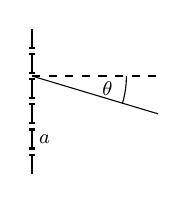
\begin{tikzpicture} [scale=0.8, transform shape]
			\draw [thick] (0,0.05) -- (0,0.35);
			\foreach \y in {0.4,0.8,1.2,1.6,2.0} {
				\draw [thick] (-0.05,\y - 0.05) -- (0.05,\y - 0.05);
				\draw [thick] (-0.05,\y + 0.05) -- (0.05,\y + 0.05);
				\draw [thick] (0,\y + 0.05) -- (0,\y + 0.35);
			}
			\draw (0.2,0.6) node {\small $a$};
			\draw [dashed] (0,1.6) -- (2,1.6);
			\draw (0,1.6) -- (2,1);
			\draw (1.5,1.6) arc (0:-17:1.5);
			\draw (1.2,1.4) node {\small $\theta$}; 
			\end{tikzpicture}
		\end{tabular} &
		\begin{mtabular}{c}
			$\fmm \sin \theta = \frac{n \lambda}{a}$
		\end{mtabular}
	\end{tabular}
\end{donotbrake}

\begin{donotbrake}
\subsection{Single slit}

\begin{tabular}{cc}
	\begin{tabular}{c}
		\begin{tikzpicture}[scale=0.7, transform shape]
			\draw [->, photon] (-1.5,1) -- (-0.7,1);
			\draw [thick] (0,-0.5) -- (0,0.7) -- (0.1,0.7) -- (0.1,-0.5);
			\draw [draw=none, fill=black!10] (0,-0.5) rectangle (0.1,0.7); 
			\draw [thick] (0,2.5) -- (0,1.3) -- (0.1,1.3) -- (0.1,2.5);
			\draw [draw=none, fill=black!10] (0,2.5) rectangle (0.1,1.3);
			\draw [|-|] (-0.2,0.7) -- (-0.2,1.3) node[pos=0.5, left] {$a$};
			\draw (2,-0.5) -- (2,2.5);
			\draw [thick, domain=-1.51:1.5, samples=150, variable=\y] plot ({30*sin(\y*200)*sin(\y*200)/((\y*20)*(\y*20)) + 2},{\y + 1}); 
			\draw (2.5,1.8) node {$I(\theta)$};
			\draw [dashed] (0,1) -- (2,1);
			\draw (0,1) -- (1.95,1.75);
			\draw (1.5,1) arc (0:21:1.5) node[pos=0.5, left] {$\theta$};
		\end{tikzpicture}
	\end{tabular} &
	\begin{mtabular}{c}
		$\fmm I(\theta) = I_0 \frac{\sin^2 \theta}{\theta^2}$ \\
		$\fmm \sin \theta = \frac{\lambda}{a}$
	\end{mtabular}
\end{tabular}
\end{donotbrake}

\subsection{Bohr-Sommerfeld equalization}

Every single particle must satisfy the following equation. The quantized energy levels below relate to the hydrogen atom

\begin{tabular}{cc}
	\begin{dtabular}
		$p$ & Momentum of particle \\
		$E_n$ & Energy of the nth state \\
		$E_{ry}$ & Rydberg Energy \\
		$a_0$ & Bohr-radius \\	
	\end{dtabular} &
	\begin{mtabular}{c}
		$\fmm \int_{length} p \cdot ds = n \cdot h \qquad n \in \mathbb{N}$ \\
		$\fmm E_n = \frac{-1}{n^2} \frac{m_e e^2}{8 \epsilon_0^2 h^2} = \frac{-1}{n^2} E_{ry} =\frac{-1}{n^2} $ \\
		$\fmm r_n = n^2 \cdot \frac{2 \epsilon_0 h}{m_e e^2} = n^2 \cdot a_0$ \\
		$E_{ry} = 13.6 \si{\electronvolt}$ \\
		$a_0 = 5.292 \cdot 10^{-11} \si{\meter}$
	\end{mtabular}
\end{tabular}

\section{Quantum Mechanics}

\begin{donotbrake}
\subsection{Wave function}
$$\psi(\vec{r}, t): \mathbb{R}^4 \rightarrow \mathbb{C} \qquad \iiint \abs{\psi(\vec{r},t)}^2 d^3r = 1 $$
$$\psi(\vec{r}, t) = a \psi_1(\vec{r},t) + b \psi_2(\vec{r}, t), \qquad \abs{a}^2 + \abs{b}^2 = 1$$
\end{donotbrake}

\begin{donotbrake}
\subsection{The Schrödinger equation}

\begin{ddtabular}
	$V(x,t)$ & potential &
	$m$ & mass \\
	$\psi(x,t)$ & 1-dimensional wave function
\end{ddtabular}

$$i \hslash \cdot \frac{\partial \psi(x,t)}{\partial t} = - \frac{\hslash^2}{2m} \cdot \frac{\partial^2 \psi(x,t)}{\partial x^2} + V(x,t) \psi(x,t)$$

\end{donotbrake}


\end{twocolumn}

\end{document}
